\lecture{10}{2025-10-11}{Processor and converter}{}
\section{Exceptions}
We we still need to do one thing which is more in the hardware side: how can we handle running multiple programs at the same time? The goal is to \textit{fool} the user into believing that the programs are running at the same time.\\
The idea on how to do that is to execute each program in small delta time, we run a program for 10ms then we stored all the value of the register somewhere, run the other program for 10 ms, store the registers value, restore the first registers values etc.\\
Another issue is also privacy on computer with multiple users, a user should not be able to go the packet that was coming because maybe this packet was for another user. What we need here is a \textit{superuser} (which will be the os) that can check at who the packet is and wether or not gives it. We need to forbid some users to do a I/Os access
\begin{center}
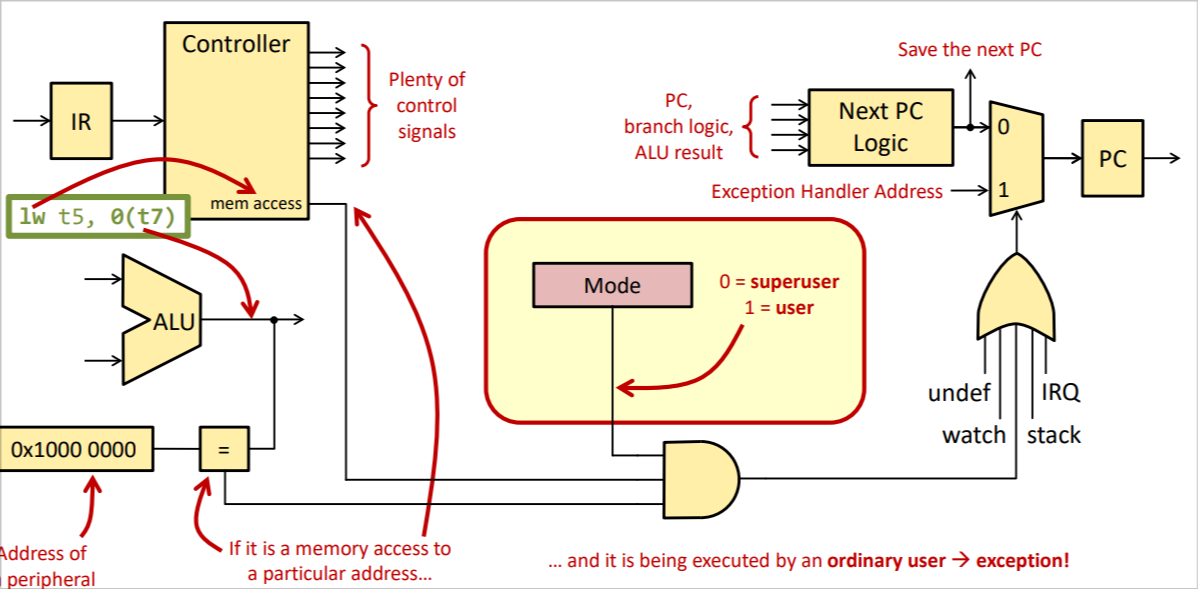
\includegraphics[scale=0.3]{screenshots/2025-10-15.png}
\end{center}
We check is the value is a memory access and it is at the place that I care $\implies$ I launch an exception. The \texttt{Mode} register is the information which allows us to know if we are the superuser or not, the implementation is \important{trivial}: adding an input at the and gate. We \important{need} two Mode otherwise we are cooked, Some questions that I found intresting during the lecture was: "\textit{isn't juste hardcode in the hardware? Why do we have only one Mode not like three or four?}".\\
But here we need an instruction to change from a mode to another, we need to be able to go    
\begin{align*} \text{user} \longleftrightarrow \text{superuser}   \end{align*}
However this is dangerous, imagine being a user being able to go to superuser and using the code of the user, when changing of user mode, we will also have to change the code that we are currenlty running.\\
But here using an exception is just a \textit{cosmetic} way of doing it, this is not an exception as the the pure sens of it.
\begin{parag}{Levels of Priviledge = Processors modes}%
\begin{itemize}
    \item Distingush \important{at least} two Processor \important{mode} :
		\begin{itemize}
		    \item \important{user mode} for the user's programs 
		    \item \important{Kernet, Supervisor, Executive}, etf for the os (kernel)
		    \item RISC-V has up to three: Machine, Supervisor, User
		\end{itemize}
		\item Have a part of the \important{processor state readable by all}, but only \important{writable with highest levels or priviledge}; at least a ;
			\begin{itemize}
			    \item Current \important{mode register}
			    \item Other configuration register (we will see some when discussing the memory hierarchy)
			\end{itemize}
			\item Method to \important{switch mode} back and forth
				\begin{itemize}
					\item A \important{dedicated instruction} to trigger a \important{software exception} and an instruction to \important{reset}
					\item RISC-V has ecal (system call) and mret sret (return from exception).
				\end{itemize}
\end{itemize}
\end{parag}
\subsubsection{Processor tasks on Exceptions}
What the processor should or could do when an exception is raised (depending on processors and type of exceptions):
\begin{itemize}
    \item Mask further interrupts 
    \item Save EPC
    \item Save information on the reason for the exception
    \item Modify privilege level (exception handler srun in some privileged mdoe)
    \item Free up some registers (e.g., copying them to shadow registers, where supported)
    \item Jump to the handler
\end{itemize}
Most or all these tasks are \important{reverted implicitly} with special instructions on exit
\begin{itemize}[noitemsep]
	\item \texttt{mret} in RISC-V reverts the privilege level and the interrupt enable
\end{itemize}
Some have to be \important{reverted explicitly by the handler}
\begin{itemize}
    \item Programmers may want to unmask further interrupts \important{as soon as it is safe}
\end{itemize}
\begin{parag}{Priorities}%
\label{par:Priorities}
We have seen that hardware \important{interrupt controllers} can help managing priotities (which interrupts is more urgent to serve?). Yet, this only affects the order IRQs are presented to the processor. But we may also want to \important{serve a high-priority interrupt while serving a lower priority one}\\
Alas, there is only one \texttt{mepc} and \texttt{mcause} register, and this is why, as soon as the processor takes an interrupt, it \important{must disable further interrupts}... What can we do?\\
\begin{itemize}
    \item Save critical information about the interrupt (\texttt{mepc, mcause, mstatus}) on some \important{same stack}, so that CSRs can be overwritten by further interrupts.
    \item Manually \important{reenable interrupts} (\texttt{mstatus}) without returning from the handler
\end{itemize}
\begin{framedremark}
The idea behind this is the same as the one when calling function and memory, we first though of having a \textbf{static} memory like here. however this won't works with recursive function for instance. What we do instead is to dynimcally allocate memory space in the stack. This is the same principle here.
\end{framedremark}
\end{parag}
\begin{parag}{Writing the handlers is very \important{very} tricky}%
\label{par:Writing the handlers is very \important{very} tricky}
Writing exception  handler is a \important{difficult task}!
\begin{itemize}
    \item Maybe the \important{stack cannot be used} (e.g., the exception results from a stack overflow)
    \item Maybe the \important{exception handler cannot be interrupted} (e.g., the handler uses static locations to save data including \texttt{mscratch}) and is therefore a nonreentrannt procedure)
    \item Maybe the \important{system cannot withstand not serving interrups} for a long time (e.g., I/Os buffers fill up)
\end{itemize}
Buggy \important{device drivers} from venders of peripherals (invoked by the interrupt handler of the operating system and running in some privileged mode) are often responsible for operating system instability.\\
\begin{framedremark}
This is why microsoft \important{formally verifies} and \important{certifies} device drivers.
\end{framedremark}
\end{parag}
\begin{parag}{Processor design Issue with Exceptions}%
\label{par:Processor design Issue with Exceptions}
Handling excpetions is \important{one of the biggest challenges} of high-performance processor design\\ Great difficulties in determining the exact state of execution and supporting a \important{precise restart mechanism}\\ 
Older processors did not support at all precise exceptions -- \important{Every exception was a terminations one,} and thus things were easy. We will seel this more in detail later in CS-200 and in eletive courses.\\
Now let us go back from what we have seen last week.
We debated if we could do something better, at the moment, to have access to the data, we were deciding when to read the data with the signal (DTACK) 

\begin{center}
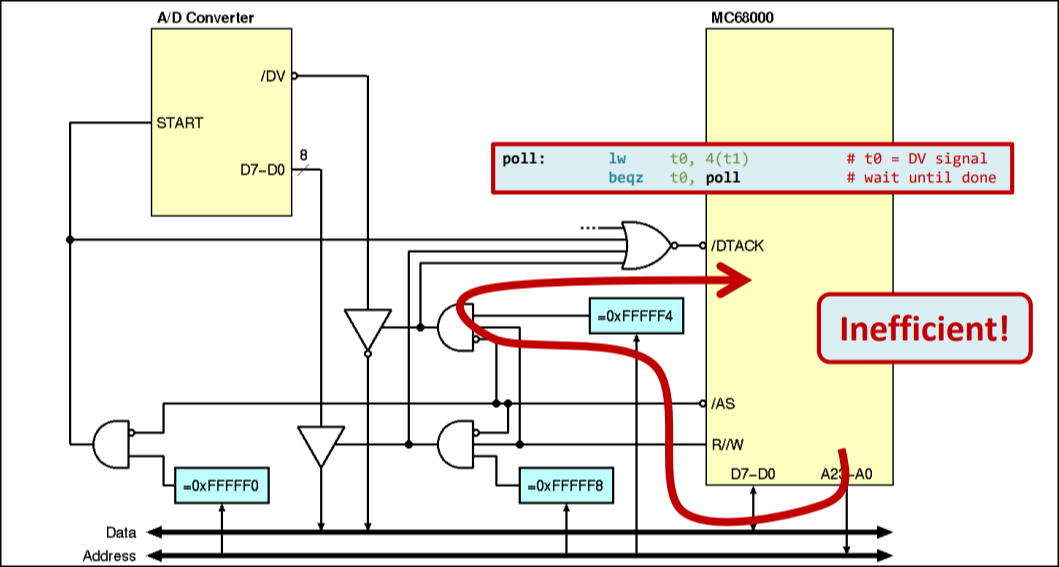
\includegraphics[scale=0.3]{screenshots/2025-10-17.png}
\end{center}
However this is pretty ineficient, the processor has to always check weither the signal is active or not instead of doing real work.\\
The goal here is to improve the interface to the A/D converter so that:
\begin{itemize}
    \item Any access (R or W) to address \texttt{oxFFFFF0} starts a new conversation 
    \item Upon completion, the A/D converter raises an interrup through the appropriate interrupt request signal of the proccessor.
    \item The result of the conversion can be ready by the processor at address\texttt{oxFFFFF8}
\end{itemize}
Suppose that our 8-bite preoccessor has an internal interrupt controller with various \texttt{IREQ}/\texttt{IACK} signap pairs for I/O interrupt requets\\
We have been assigned for our ADC these:
\begin{itemize}
    \item \texttt{IREQ3}: input,, dedicated to our peripheral to request attention
    \item \texttt{IACK3} output; used by the processor to signal to our peripheral that the request is acknowledged and is being served
\end{itemize}
\begin{center}
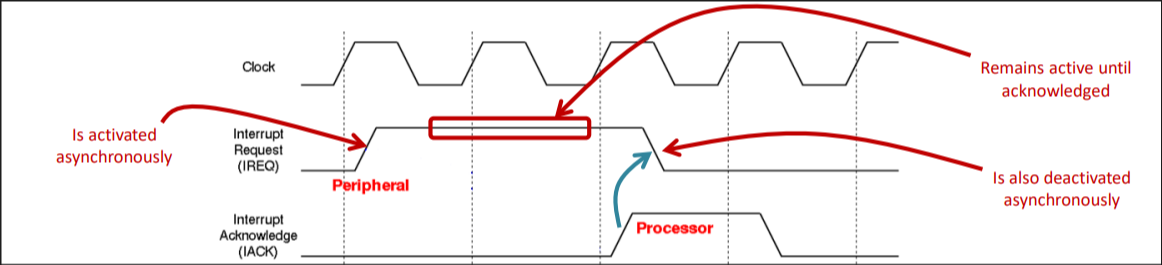
\includegraphics[scale=0.3]{screenshots/2025-10-17_1.png}
\end{center}
There is two main things here to acknowledged:\\
First, what we can see is that between the IREQ and the processor responds, we don't have a clock edge, this means that the acknowledged is only combination logic here.\\
On the other hand, we also see here that the IREQ here stays up until it is acknowledged, this means that we need to store the "up state"  for more than one clock cycle. What does this means? $\implies $ \important{flip flop}, we will ne a flip flop that store this information for us. What is weird about this flip flop is that the input that is store in it is 1, not the input value. The one deciding when it goes up or not is the A/D converter. This is looking very ugly\ldots 
\begin{center}
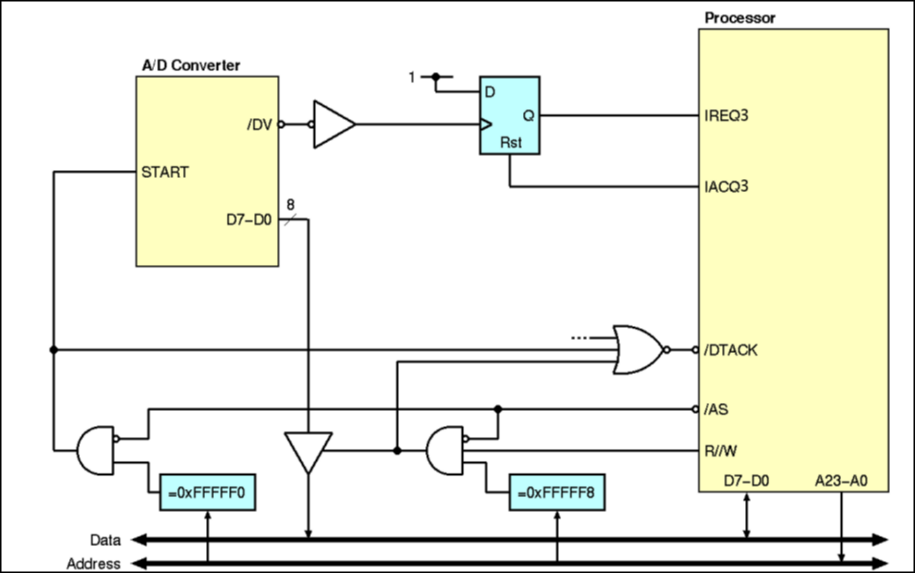
\includegraphics[scale=0.3]{screenshots/2025-10-17_2.png}
\end{center}
But why is this an error in any other context forbidden?\\
$\implies $ any flip flop \important{must} be connected to the clock of the system.

\end{parag}

\begin{parag}{A/D converter: startADC}
	this is a pretty trivial task to do
	\begin{lstlisting}[language={[RISC-V]Assembler}]
	startADC:	lui t0, 0xfff
				addi t0, t0, 0xff0 # to = 0xfffff0
				sw zero, 0(t0)

				ret
	\end{lstlisting}
\end{parag}
\begin{parag}{Handler}
    On the other hand the handler part is a bit harder.\\
	For instance the handler:\\
	
	\begin{lstlisting}[language={[RISC-V]Assembler}]
startADC:	addi sp, sp, --
			..
			..
			csrr t0, mcause

			..
			jal readADC
			jal buffer #we need to store the information somewhere for other to have access to it
			..
			mret
	
	\end{lstlisting}
	\begin{framedremark}
	The \texttt{mcause} is the register which stores the machine external interrupt
	\end{framedremark}
	So the real part for this is:
	\begin{lstlisting}[language={[RISC-V]Assembler}]
handler:	addi sp, sp, -120 # save all registers but zero and sp
			sw x1, 0(sp)
			sw x3, 4(sp)
			.. etc ..
			sw x31, 116(sp)

			csrr s0, mcause # Read exception cause
			bgez so, handleException #branche if not an interrupt (MSB = 0, looks like zero or a positive number..)
			slli s0, s0, 1 # Get rid ofthe MSB of s0, so that what is left is the cause
			srli s0, s0, 1 
			li s1, 11 
			bne s1, s2, handleOtherInts # Branch if not an external interrupt

			jal readADC  # return a0 = ADC result 
			jal insertIntoBuffer  # Gets a0 = value to add to a circular buffer

restore:	lw x1, 0(sp)
			lw x3, 4(sp)
			.. etc ..
			lw x31, 116(sp)

			addi sp, sp, 120
			mret
	\end{lstlisting}
	
\end{parag}
\begin{parag}{A/D converter: insertIntoBuffer}
	\begin{lstlisting}[language={[RISC-V]Assembler}]
.section .data 	
		.equ bufferSize, 1024 #define buffer size 
		.equ bufferBytes, bufferSize * 4 # compute the total size in bytes for the buffer 

bufferPointer: 	.word 0  # Initializse the pointer index to 02d
buffer: 		.space bufferBytes  # Allocate space for bufferSize * wordsize bytes

.section .text 
insertIntoBuffer: 	
	la t0, la t0 bufferPointer # Load address of budderPointer into t0
	lw t1, 0(t0) # Load current buffer pointer into t1
	la t2, buffer  # Load base address of the buffer into t2
	slli t3, t1, 2  # Multiply
	add t4, t2, t3 
	sw a0, 0(t4)
	addi t1, t1, 1 
	li t5, bufferSize - 1 
	and t1, t1, t5 
	sw t1, 0(t0)

	ret
\end{lstlisting}
\end{parag}








